\subsection{Cantilever beam}
\paragraph{}
A two-dimensional cantilever beam subjected to a parabolic shear load at the free end is examined as shown in Fig.~\ref{iso_fig:cantilever_beam_geo_bc}.
    \begin{figure}[h!]
    \centering
        \scalebox{0.8}{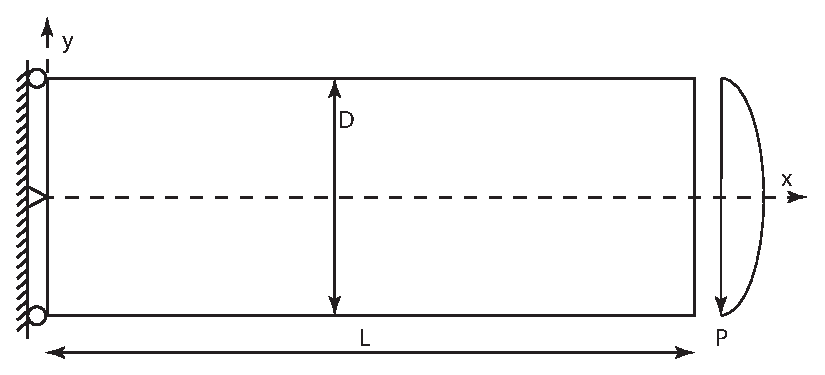
\includegraphics{isogeometric_sbfem/images/cantilever_beam_geo_bc.eps}}
        \caption{ Cantilever beam: Geometry and boundary conditions.}
        \label{iso_fig:cantilever_beam_geo_bc}
    \end{figure}
%
The geometry is: length $ L = \SI{8}{\meter} $, height $ D = \SI{4}{\meter} $.
The material properties are: Young’s modulus $ E = \SI{3e7}{\newton \per \square \meter}$ , Poisson’s ratio $ \nu = 0.25 $.
The parabolic shear force is $P = \SI{250}{\meter} $.
The exact solutions for the displacements are given by \citep{Aug2008}:
    \begin{equation}
        \begin{aligned}
            u(x,y) &= 
                \frac{Py}{6 \mean{E} I}
                \left[
                    \left(
                        6L-3x
                    \right)x
                    +\left(
                        2+ \mean{\nu}
                    \right)\left(
                        y^2-\frac{D^2}{4}
                    \right)
                \right]
            \\
            v(x,y) &=  
                -\frac{P}{6 \mean{E} I}
                \left[
                    3 \mean{\nu} y^2 \left(
                        L-x
                    \right)+
                    \left(
                        4+5 \mean{\nu}
                    \right)\frac{D^2x}{4}+
                    \left(
                        3L-x
                    \right)x^2
                \right]        
        \end{aligned}
    \label{iso_eq:cantilever_beam_displacement_solution}
    \end{equation}
%
where $I=D^3/12$ is the moment of inertia, $\mean{E}=E$, $\mean{\nu}=\nu$ and $\mean{E}=E/(1-\nu^2)$, $\mean{\nu}=\nu/(1-\nu)$ for plane stress and plane strain condition respectively.
The stress $\sigma$ can be expressed as \citep{Aug2008}
    \begin{subequations}
    \begin{align}
        \sigma_{xx} &= \frac{P(L-x)y}{I} \\
        \sigma_{yy} &= 0 \\
        \tau_{xy} &= -\frac{P}{2I} \left[
            \frac{D^2}{4} - y^2
        \right]
    \end{align}
    \label{iso_eq:cantilever_beam_stress_solution}
    \end{subequations}
%
The strain energy can be derived from Eq.~\ref{iso_eq:cantilever_beam_stress_solution} and Eq.~\ref{iso_eq:cantilever_beam_displacement_solution} as
\begin{equation}
\epsilon = 
    \frac{1}{2} \left(
        \frac{D^3 L^3 P^2}{36EI^2} + 
        \frac{D^5LP^2(1+v)}{60EI^2}
    \right)
    \label{iso_eq:cantilever_beam_energy_solution}
\end{equation}
\paragraph{}
In this example, rigid body motion is constrained by fixing 3 DOF on the left edge of the beam.
$u_x=0$ for points at $(0,-D/2)$ and $(0,D/2)$ and $u_y =0$ for point at $(0,0)$.
Surface tractions determined from the analytical solution of stress in Eq.~\ref{iso_eq:cantilever_beam_stress_solution} are applied on the boundary.

\paragraph{}
From the description in Section~\ref{iso_section:surface_traction}, the expression of the surface tractions must be transformed into NURBS-like representation before they can be applied.
The control points that describe a second order function as surface tractions in this example can be solved mathematically.
Assume the knot vector is evenly spaced and the shape functions is in second order, i.e. knot vector $\Xi=[0,0,0,1,1,1]$.
Weight vector will be uniform because only the straight line is being interpolated, i.e. weight vector $w=[1,1,1]$.
Three basis functions used in B-Spline will be
    \begin{equation}
    \begin{aligned}
        N_1 & = (1-u)^2 \\
        N_2 & = 2u(1-u) \\
        N_3 & = u^2
    \end{aligned}
    \end{equation}
%
With the given targeted parabola as $y=ax^2+bx+c,x \in [0,1]$, the generalized control points for the NURBS curve will be
    \begin{equation}
        P= \begin{bmatrix}
            P_x \\
            P_y
        \end{bmatrix} = \begin{bmatrix}
            0 & m & 1 \\
            c & n & a+b+c
        \end{bmatrix}
    \end{equation}
%
where $m$ and $n$ are unknowns for the second control point.
B-spline curve $C=[N][P]$ then can be expressed as in parametric form as
    \begin{equation}
        \left\{
        \begin{aligned}
            x &= 2u(1-u)m + u^2 \\
            y &= c(1-u)^2 + 2u(1-u)n + (a+b+c)u^2
        \end{aligned}
        \right.
    \label{iso_eq:parabola_fitting_parametric}
    \end{equation}
%
After substituting Eq.~\ref{iso_eq:parabola_fitting_parametric} into $y=ax^2+bx+c$, we then have the system of equations as
    \begin{equation}
        \begin{bmatrix}
            0 \\
            0 \\
            2c - 2n +a +b \\
            2n - 2c \\
            c
        \end{bmatrix} = 
        \begin{bmatrix}
            4am^2-4am+a \\
            -8am^2 + 4am \\
            4am^2 -2bm +b \\
            2bm \\
            c
        \end{bmatrix}
    \end{equation}
%
$m$ and $n$ then can be solved as
    \begin{equation}
        \left\{
        \begin{aligned}
            m &= \frac{1}{2} \\
            n &= \frac{b+2c}{2}
        \end{aligned}
        \right.
    \end{equation}
%
The numerical convergence of the relative error in the displacement norm and the relative error in the energy norm are shown in Fig.~\ref{iso_fig:cantilever_beam_convergence} for various order of NURBS basis functions with refinement.
Fig.~\ref{iso_fig:cantilever_beam_convergence} also shows the error in the displacement norm when quadratic Lagrange shape functions are used along each edge within the scaled boundary formulation.
It can be observed that NURBS basis functions yield superior accuracy when compared to Lagrange basis functions of the same order.
It is seen that as the order of the shape functions is increased, the error decreases while the convergence rate increases.
\begin{figure}
    \begin{subfigure}[b]{1\linewidth}
        \centering
        \scalebox{0.7}{
            % This file was created by matlab2tikz v0.4.6 running on MATLAB 8.2.
% Copyright (c) 2008--2014, Nico Schlömer <nico.schloemer@gmail.com>
% All rights reserved.
% Minimal pgfplots version: 1.3
% 
% The latest updates can be retrieved from
%   http://www.mathworks.com/matlabcentral/fileexchange/22022-matlab2tikz
% where you can also make suggestions and rate matlab2tikz.
% 
\begin{tikzpicture}

\begin{axis}[%
width=4.52083333333333in,
height=3.5146875in,
scale only axis,
xmode=log,
xmin=10,
xmax=1000,
xminorticks=true,
xlabel={Total DOF},
ymode=log,
ymin=1e-05,
ymax=1,
yminorticks=true,
ylabel={Error},
title={l2l Displacement  Error},
legend style={draw=black,fill=white,legend cell align=left}
]
\addplot [color=blue,solid,mark=square,mark options={solid}]
  table[row sep=crcr]{
20	0.223473837	\\
40	0.0493	\\
80	0.011281049	\\
160	0.00266076	\\
};
\addlegendentry{1st order};

\addplot [color=black!50!green,solid,mark=o,mark options={solid}]
  table[row sep=crcr]{
20	0.067810872	\\
40	0.003190002	\\
80	0.000250473	\\
160	2.27e-05	\\
};
\addlegendentry{2nd order};

\addplot [color=red,solid,mark=+,mark options={solid}]
  table[row sep=crcr]{
20	0.0713	\\
40	0.00707	\\
80	0.000688	\\
160	8.85e-05	\\
};
\addlegendentry{LNGL 2nd order};

\end{axis}
\end{tikzpicture}%
        }
        \label{iso_fig:cantilever_beam_displacement_convergence}
        \caption{the relative error in displacement norm $(L^2)$}
    \end{subfigure}
    
    \begin{subfigure}[b]{1\linewidth}
        \centering
        \scalebox{0.7}{
            % This file was created by matlab2tikz v0.4.6 running on MATLAB 8.2.
% Copyright (c) 2008--2014, Nico Schlömer <nico.schloemer@gmail.com>
% All rights reserved.
% Minimal pgfplots version: 1.3
% 
% The latest updates can be retrieved from
%   http://www.mathworks.com/matlabcentral/fileexchange/22022-matlab2tikz
% where you can also make suggestions and rate matlab2tikz.
% 
\begin{tikzpicture}

\begin{axis}[%
width=4.52083333333333in,
height=3.5146875in,
scale only axis,
xmode=log,
xmin=10,
xmax=1000,
xminorticks=true,
xlabel={Total DOF},
ymode=log,
ymin=0.001,
ymax=1,
yminorticks=true,
ylabel={Error},
title={l2l Strain Energy  Error},
legend style={draw=black,fill=white,legend cell align=left}
]
\addplot [color=blue,solid,mark=square,mark options={solid}]
  table[row sep=crcr]{
20	0.701427116670007	\\
40	0.417133072292284	\\
80	0.228254244210267	\\
160	0.119582607431014	\\
};
\addlegendentry{1st order};

\addplot [color=black!50!green,solid,mark=o,mark options={solid}]
  table[row sep=crcr]{
20	0.180496573374677	\\
40	0.02575787258296	\\
80	0.0046690470119715	\\
160	0.0010295630140987	\\
};
\addlegendentry{2nd order};

\addplot [color=red,solid,mark=+,mark options={solid}]
  table[row sep=crcr]{
20	0.304275389	\\
40	0.065	\\
80	0.014502273	\\
160	0.003385053	\\
};
\addlegendentry{LNGL 2nd order};

\end{axis}
\end{tikzpicture}%
        }
        \label{iso_fig:cantilever_beam_energy_convergence}
        \caption{the relative error in the energy norm}
    \end{subfigure}
\caption{Bending of thick cantilever beam: Convergence results}
\label{iso_fig:cantilever_beam_convergence}
\end{figure}
%
